\subsubsection{Signal source}
Raw I/Q samples of each channel, as recorded (0.5~s analysed, from 10~s into the recording).

\begin{figure}[H]
  \centering
  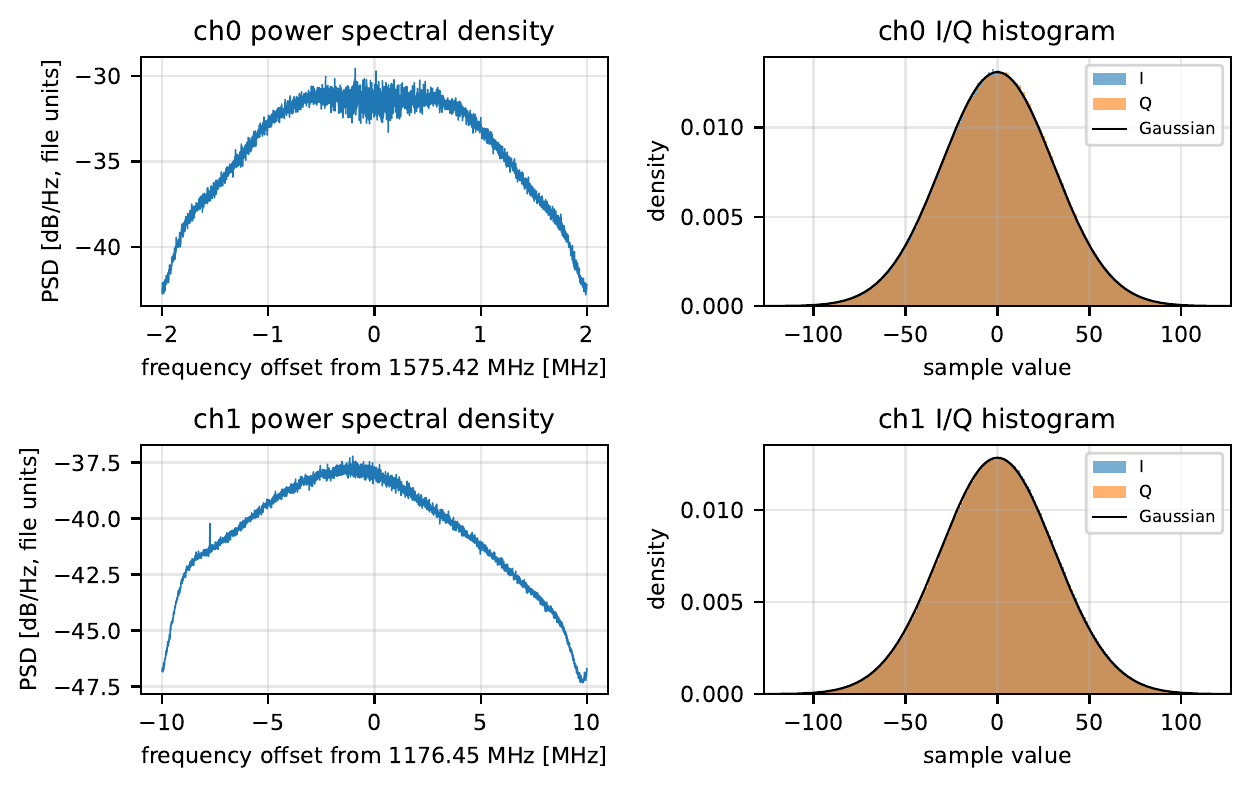
\includegraphics[width=1.0\linewidth]{gnss_sdr/x310_20261022T190000Z/source.png}
  \caption{Signal source: power spectral density (the receiver passband over a flat thermal-noise floor; GNSS signals are below the noise, so only interference would stand out) and I/Q histograms (Gaussian noise, centred, not clipped).}
\end{figure}

\begin{table}[H]
  \centering
  \footnotesize
  \resizebox{\ifdim\width>\linewidth\linewidth\else\width\fi}{!}{%
  \begin{tabular}{lcc}
    \hline
    \textbf{Channel} & \textbf{ch0} & \textbf{ch1} \\
    \hline
    Frequency [MHz] & 1575.42 & 1176.45 \\
    Rate [MS/s] & 4 & 20 \\
    Format & ci8 & ci8 \\
    Gain [dB] & 25 & 25 \\
    Std I / Q & 30.4 / 30.5 & 31.1 / 31.1 \\
    Mean I / Q & -0.26 / 0.20 & 0.26 / -0.07 \\
    Clipped [\%] & 0.003 & 0.004 \\
    Lost samples & 2,912 & 14,924 \\
    \hline
  \end{tabular}}
  \caption{Signal source: sample statistics per channel.}
\end{table}

\subsubsection{Signal conditioner}
How each recorded channel is turned into the complex baseband stream the channels process.

\begin{table}[H]
  \centering
  \footnotesize
  \resizebox{\ifdim\width>\linewidth\linewidth\else\width\fi}{!}{%
  \begin{tabular}{lcc}
    \hline
    \textbf{Channel} & \textbf{ch0 (L1 C/A)} & \textbf{ch1 (L5)} \\
    \hline
    File format & ci8 & ci8 \\
    Source item type & ibyte & ibyte \\
    Data type adapter & Ibyte\_To\_Complex & Ibyte\_To\_Complex \\
    Input filter & Pass\_Through & Pass\_Through \\
    Resampling & \$\textbackslash{}times\$5 zero-order hold (offline) & Pass\_Through \\
    Rate [MS/s] & 4 $\to$ 20 & 20 $\to$ 20 \\
    \hline
  \end{tabular}}
  \caption{Signal conditioner: recorded format and rate to gnss-sdr's internal \texttt{gr\_complex} stream; both bands are read in lockstep by one \texttt{Multichannel\_File\_Signal\_Source}.}
\end{table}

\subsubsection{Acquisition}
Two-dimensional search over code delay and Doppler (one channel per band dumped; the others behave alike).

\begin{figure}[H]
  \centering
  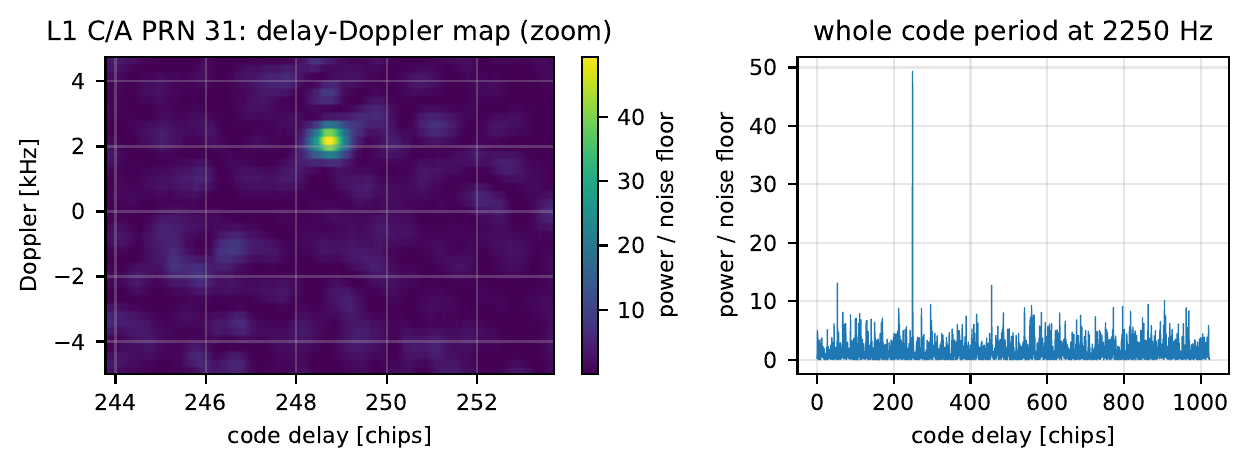
\includegraphics[width=1.0\linewidth]{gnss_sdr/x310_20261022T190000Z/acq_1C.png}
  \caption{Acquisition, L1 C/A: delay--Doppler search of PRN 31; one sharp peak (test statistic 71 vs threshold 47) at 2250~Hz and 248.7~chips.}
\end{figure}

\begin{figure}[H]
  \centering
  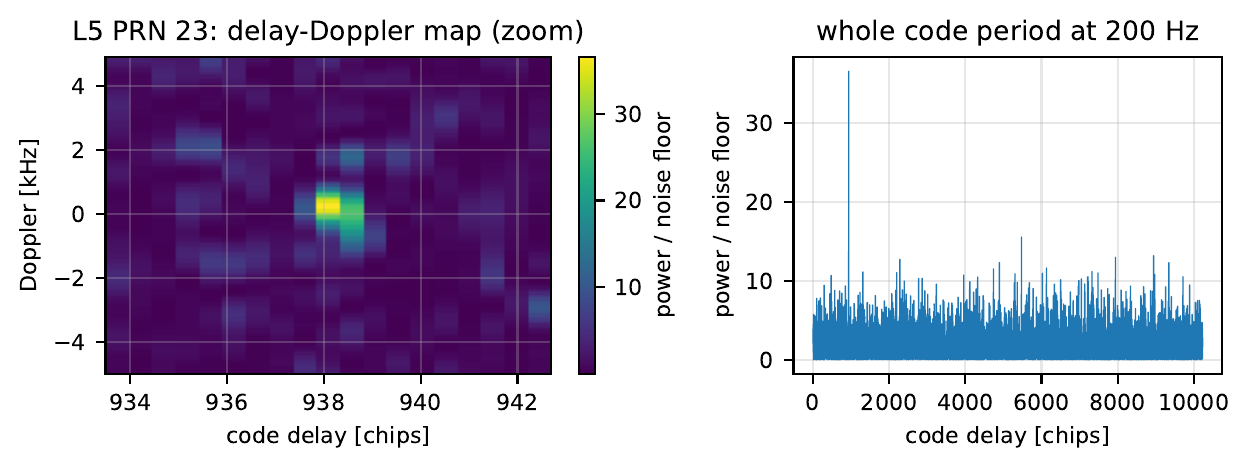
\includegraphics[width=1.0\linewidth]{gnss_sdr/x310_20261022T190000Z/acq_L5.png}
  \caption{Acquisition, L5: delay--Doppler search of PRN 23; one sharp peak (test statistic 51 vs threshold 49) at -1587~Hz and 938.1~chips.}
\end{figure}

\begin{table}[H]
  \centering
  \footnotesize
  \resizebox{\ifdim\width>\linewidth\linewidth\else\width\fi}{!}{%
  \begin{tabular}{lrrrr}
    \hline
    \textbf{Band} & \textbf{Attempts} & \textbf{Detections} & \textbf{Detected PRNs} & \textbf{Best statistic / threshold} \\
    \hline
    L1 C/A & 11 & 1 & 31 & 1.5 \\
    L5 & 115 & 1 & 23 & 1.0 \\
    \hline
  \end{tabular}}
  \caption{Acquisition: search attempts of the dumped channel. Attempts on satellites that are not in view (or, for L5/L2C, do not broadcast that signal) are rejected below the threshold.}
\end{table}

\subsubsection{Tracking}
Code (DLL) and carrier (PLL) loops per satellite.

\begin{figure}[H]
  \centering
  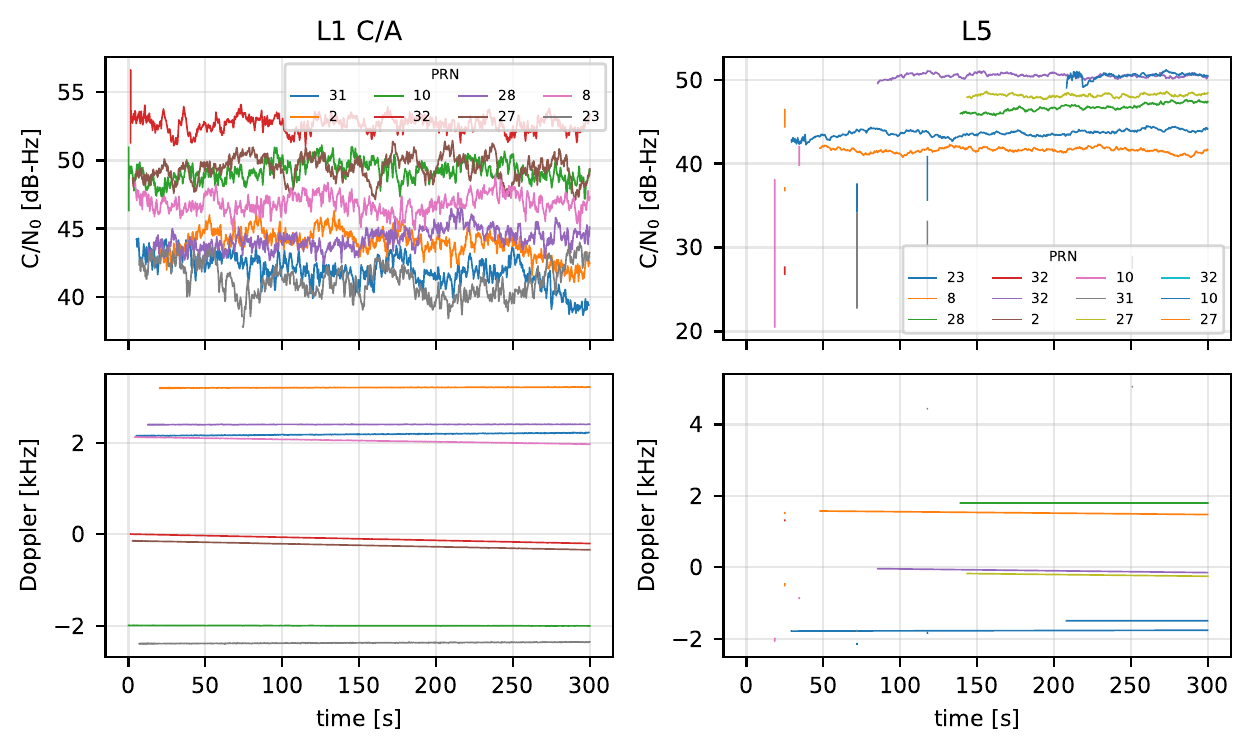
\includegraphics[width=1.0\linewidth]{gnss_sdr/x310_20261022T190000Z/tracking.png}
  \caption{Tracking: carrier-to-noise density ratio and carrier Doppler per satellite, while phase-locked (smooth Doppler curves = loops following the real satellite motion).}
\end{figure}

\begin{figure}[H]
  \centering
  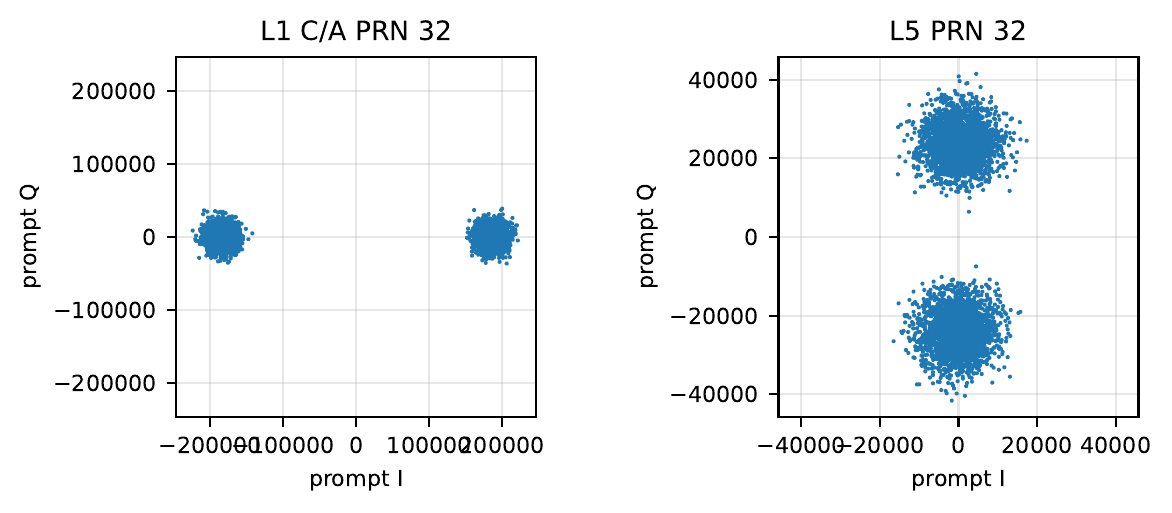
\includegraphics[width=1.0\linewidth]{gnss_sdr/x310_20261022T190000Z/tracking_iq.png}
  \caption{Tracking: prompt correlator outputs of the strongest satellite per band. Two tight clusters on one axis (the $\pm1$ data bits; GNSS-SDR's L5 tracking puts the data component on the Q axis) mean the PLL is phase-locked; a ring would mean it is not.}
\end{figure}

\begin{table}[H]
  \centering
  \footnotesize
  \resizebox{\ifdim\width>\linewidth\linewidth\else\width\fi}{!}{%
  \begin{tabular}{lrrrrrr}
    \hline
    \textbf{Band} & \textbf{Ch.} & \textbf{PRN} & \textbf{Median C/N$_0$ [dB-Hz]} & \textbf{Phase-locked [\%]} & \textbf{Losses of lock} & \textbf{Tracked [s]} \\
    \hline
    L1 C/A & 0 & 31 & 42.7 & 93 & 0 & 561 \\
    L1 C/A & 1 & 2 & 43.5 & 95 & 0 & 28 \\
    L1 C/A & 2 & 10 & 49.2 & 100 & 0 & 512 \\
    L1 C/A & 3 & 32 & 52.9 & 100 & 0 & 30 \\
    L1 C/A & 4 & 28 & 43.8 & 93 & 0 & 526 \\
    L1 C/A & 5 & 27 & 49.0 & 94 & 0 & 528 \\
    L1 C/A & 6 & 8 & 47.0 & 92 & 0 & 30 \\
    L1 C/A & 7 & 23 & 41.9 & 92 & 0 & 530 \\
    L5 & 8 & 23 & 43.5 & 95 & 0 & 372 \\
    L5 & 9 & 8 & 41.7 & 67 & 0 & 374 \\
    L5 & 10 & 28 & 46.4 & 58 & 1 & 279 \\
    L5 & 10 & 32 & 28.9 & 0 & 1 & 16 \\
    L5 & 11 & 32 & 50.4 & 66 & 0 & 327 \\
    L5 & 12 & 2 & 28.8 & 0 & 1 & 16 \\
    L5 & 13 & 10 & 29.2 & 1 & 5 & 32 \\
    L5 & 13 & 31 & 28.7 & 0 & 5 & 48 \\
    L5 & 14 & 27 & 48.2 & 56 & 1 & 279 \\
    L5 & 14 & 32 & 28.9 & 0 & 1 & 16 \\
    L5 & 15 & 10 & 32.2 & 36 & 3 & 51 \\
    L5 & 15 & 27 & 28.8 & 0 & 3 & 16 \\
    \hline
  \end{tabular}}
  \caption{Tracking: per channel and satellite (phase-locked: carrier lock test $> 0.8$).}
\end{table}

\subsubsection{Telemetry decoder}
Navigation-message decoding: bit/frame synchronization, parity/CRC, the ephemeris, and the satellite transmit time (time of week) of every measurement.

\begin{figure}[H]
  \centering
  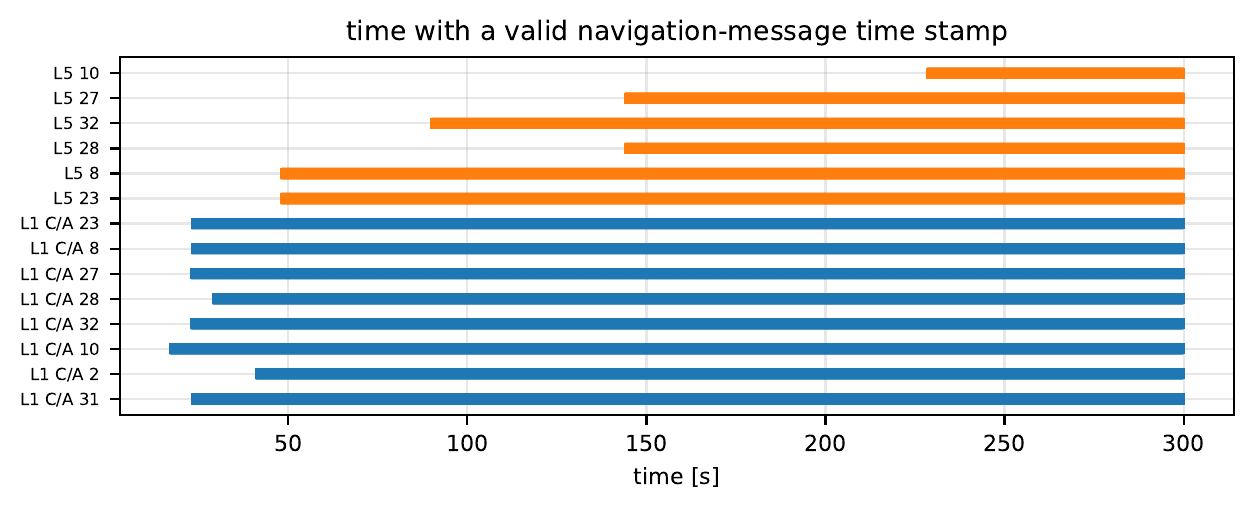
\includegraphics[width=1.0\linewidth]{gnss_sdr/x310_20261022T190000Z/telemetry.png}
  \caption{Telemetry decoder: per band and satellite, when the decoder delivered a valid transmit time (the first one comes after the first complete frame/message).}
\end{figure}

\begin{table}[H]
  \centering
  \footnotesize
  \resizebox{\ifdim\width>\linewidth\linewidth\else\width\fi}{!}{%
  \begin{tabular}{lrrrrr}
    \hline
    \textbf{Band} & \textbf{PRN} & \textbf{Messages decoded} & \textbf{Ephemeris} & \textbf{First valid at [s]} & \textbf{TOW [s]} \\
    \hline
    L1 C/A & 2 & 44 & yes & 41.1 & 414066.0 \\
    L1 C/A & 8 & 46 & yes & 23.1 & 414048.0 \\
    L1 C/A & 10 & 48 & yes & 17.1 & 414042.0 \\
    L1 C/A & 23 & 46 & yes & 23.1 & 414048.0 \\
    L1 C/A & 27 & 47 & yes & 23.1 & 414048.0 \\
    L1 C/A & 28 & 44 & yes & 29.1 & 414054.0 \\
    L1 C/A & 31 & 47 & yes & 23.1 & 414048.0 \\
    L1 C/A & 32 & 47 & yes & 23.1 & 414048.0 \\
    L5 & 8 & 25 & yes & 48.1 & 414073.0 \\
    L5 & 10 & 7 & yes & 228.4 & 414253.3 \\
    L5 & 23 & 31 & yes & 48.1 & 414073.0 \\
    L5 & 27 & 15 & yes & 144.1 & 414169.0 \\
    L5 & 28 & 19 & yes & 144.1 & 414169.0 \\
    L5 & 32 & 22 & yes & 90.0 & 414114.9 \\
    \hline
  \end{tabular}}
  \caption{Telemetry decoder: L1 C/A LNAV subframes and L2C/L5 CNAV messages decoded, ephemeris obtained, and the first valid time of week.}
\end{table}

\subsubsection{Observables}
Pseudorange, carrier phase and Doppler of every channel at common receiver epochs.

\begin{figure}[H]
  \centering
  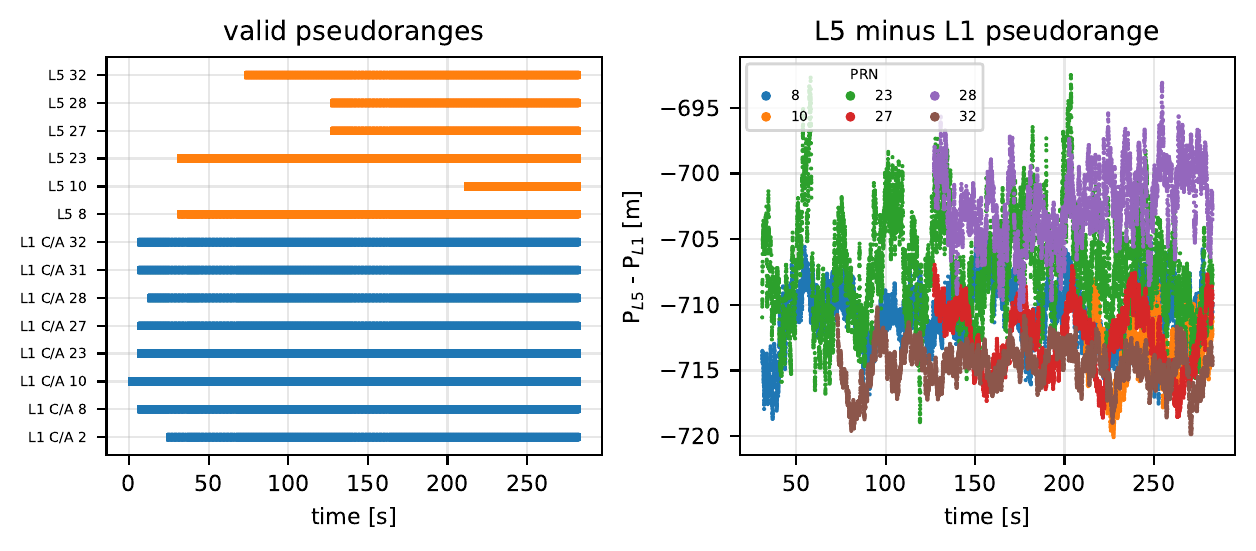
\includegraphics[width=1.0\linewidth]{gnss_sdr/x310_20261022T190000Z/observables.png}
  \caption{Observables: epochs with a valid pseudorange per band and satellite, and the difference between the two bands' pseudoranges of the same satellite (a constant receiver inter-band bias, the same for every satellite, plus the slowly varying ionospheric delay).}
\end{figure}

\begin{table}[H]
  \centering
  \footnotesize
  \resizebox{\ifdim\width>\linewidth\linewidth\else\width\fi}{!}{%
  \begin{tabular}{lrrrrr}
    \hline
    \textbf{PRN} & \textbf{Common epochs} & \textbf{of run [\%]} & \textbf{Mean [m]} & \textbf{Std [m]} & \textbf{Drift [m/s]} \\
    \hline
    8 & 12228 & 82 & -710.75 & 2.19 & 0.0014 \\
    10 & 3563 & 24 & -713.39 & 2.20 & 0.0208 \\
    23 & 12231 & 82 & -707.12 & 3.91 & 0.0006 \\
    27 & 7627 & 51 & -712.62 & 2.45 & -0.0107 \\
    28 & 7628 & 51 & -702.35 & 2.80 & 0.0221 \\
    32 & 10330 & 69 & -714.67 & 1.54 & -0.0003 \\
    \hline
  \end{tabular}}
  \caption{Observables: P$_{\mathrm{L5}}$ $-$ P$_{\mathrm{L1}}$ per satellite at common epochs (similar means = shared receiver bias; std = code noise of both bands).}
\end{table}

\subsubsection{PVT}
Position from the pseudoranges and the decoded ephemeris, compared with the surveyed antenna position (-23.209433$^\circ$, -45.874875$^\circ$, 596.42~m).

\begin{figure}[H]
  \centering
  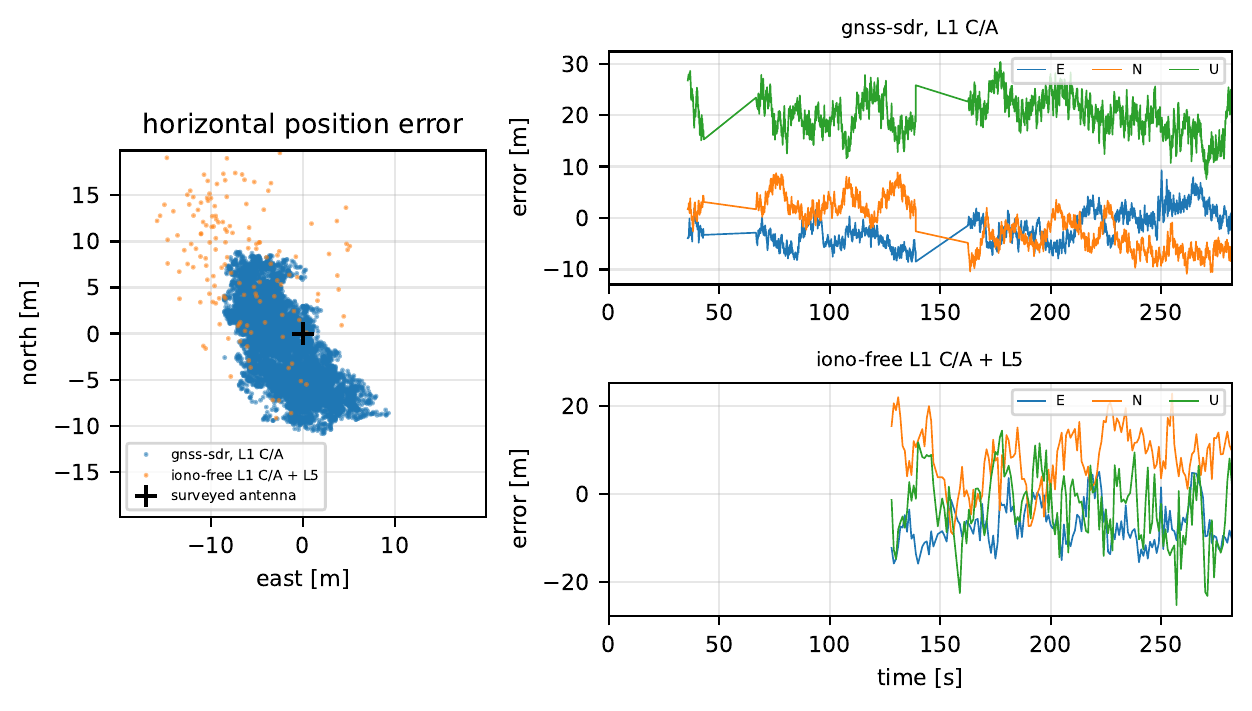
\includegraphics[width=1.0\linewidth]{gnss_sdr/x310_20261022T190000Z/pvt.png}
  \caption{PVT: position error with respect to the surveyed antenna position. L1 C/A: gnss-sdr's own solution (broadcast ionosphere model). Iono-free: computed from gnss-sdr's observables and decoded ephemeris (gnss\_spp.py), removing the ionospheric delay with the second band (pseudoranges carrier-smoothed over 100~s).}
\end{figure}

\begin{figure}[H]
  \centering
  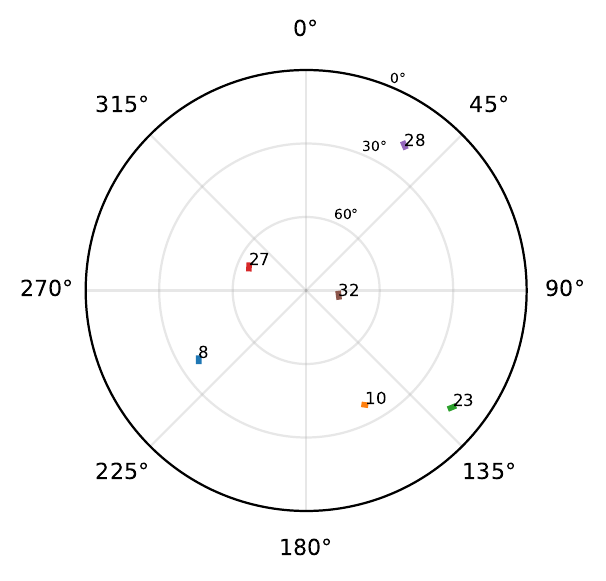
\includegraphics[width=0.45\linewidth]{gnss_sdr/x310_20261022T190000Z/skyplot.png}
  \caption{PVT: sky plot of the satellites in the dual-frequency solution (azimuth, elevation) during the recording.}
\end{figure}

\begin{table}[H]
  \centering
  \footnotesize
  \resizebox{\ifdim\width>\linewidth\linewidth\else\width\fi}{!}{%
  \begin{tabular}{lcc}
    \hline
    \textbf{Solution} & \textbf{gnss-sdr, L1 C/A} & \textbf{iono-free L1 C/A + L5} \\
    \hline
    Solutions & 10332 & 151 \\
    Run with fix [\%] & 72 & 54 \\
    Mean E / N / U [m] & -2.0 / -1.5 / 20.0 & -7.0 / 8.2 / -2.9 \\
    Std E / N / U [m] & 3.2 / 4.5 / 3.6 & 5.0 / 6.7 / 7.9 \\
    RMS 2-D [m] & 6.1 & 13.6 \\
    RMS 3-D [m] & 21.2 & 16.0 \\
    95\% horiz. [m] & 9.3 & 20.6 \\
    \hline
  \end{tabular}}
  \caption{PVT: position error statistics with respect to the surveyed antenna (mean = accuracy, std = precision; \% of the run's seconds with a position; gnss-sdr outputs several solutions per second, the iono-free one is computed once per second).}
\end{table}

